%%%% Paramétrage du cours %%%%
\def\xxactivite{Cours}
\def\xxauteur{\textsl{Xavier Pessoles}}

\fichefalse
\proftrue
\tdfalse
\courstrue

\def\xxnumchapitre{Chapitre 1 \vspace{.2cm}}
\def\xxchapitre{\hspace{.12cm} Introduction aux méthodes numériques}

\def\xxcompetences{%
\textsl{%
\textbf{Savoirs et compétences :}\\
\begin{itemize}[label=\ding{112},font=\color{ocre}] 
\item B2-12 : proposer un modèle cinématique à partir d'un système réel ou d'une maquette numérique;
\item B2-15 : Simplifier un modèle de mécanisme.
\end{itemize}
}}


\def\xxfigures{
%\includegraphics[width=0.6\textwidth]{lola}\\
%\textit{Robot humanoïde Lola}

}%figues de la page de garde%figues de la page de garde

\input{\repStyle/new_pagegarde}
\vspace{2cm}
\pagestyle{fancy}
\thispagestyle{plain}


\section{Equations stationnaires -- Résolution de $f(x)=0$}

\subsection{Principe de la méthode de dichotomie}

\begin{theorem}
\textbf{Théorème des valeurs intermédiaires}

Soit $f$ une fonction définie et continue sur l'intervalle $[a,b]$ à valeur dans $\mathbb{R}$. Pour tout $u\in[f(a),f(b)]$, il existe au moins un réel $c\in [a,b]$  tel que $f(c)=u$.

 En particulier (Théorème de Bolzano), si $f(a)$ et $f(b)$ sont de signes différents, il existe au moins un réel $c$ tel que $f(c)=0$. 
\end{theorem}

\begin{minipage}[c]{.6\linewidth}
Ainsi, pour une fonction donnée définie sur un intervalle donné, le but de l'algorithme de dichotomie va être de découper en 2 l'intervalle [a,b] en deux, afin d'y trouver la solution. Par divisions successives de l'intervalle, on convergera vers la solution.

\begin{rem}
\textbf{Tester le signe de $f(a)$ et $f(b)$.}

Il existe plusieurs méthodes pour tester si $f(a)$ et $f(b)$ sont de signes différents. Si on ne se préoccupe pas de savoir la relation d'ordre entre $f(a)$ et $f(b)$, un test efficace consiste en un test du signe de $f(a)\cdot f(b)$. 
\end{rem}

\end{minipage} \hfill
\begin{minipage}[c]{.35\linewidth}
\begin{center}
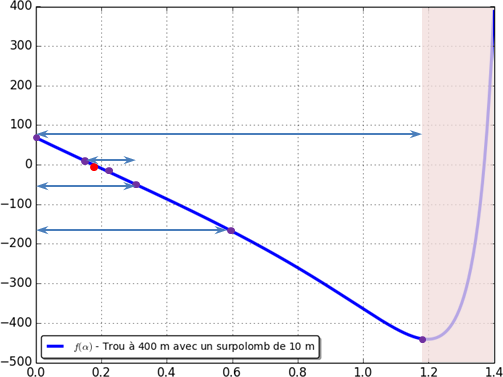
\includegraphics[width=\linewidth]{InterpretationG}
\end{center}
\end{minipage}

\subsection{Principe de la méthode de Newton}
\begin{theorem}
\textbf{Développement de Taylor à l'ordre 1}

Soit $f$ une fonction $C^1$ sur un intervalle $I$ et $a\in I$. Le développement de Taylor à l'ordre 1 de $f$ est donné par 
$$
f(x)=f(a)+ f'(a)\cdot(x-a)+\mathit{o}(x-a)
$$
\end{theorem}


\begin{minipage}[c]{.6\linewidth}
Géométriquement, lorsqu'on néglige le reste, le développement de Taylor donne l'équation de la tangente en $a$. Notons $\Delta(x)$ cette équation.

L'abscisse $c$ de l'intersection de la tangente avec l'axe des abscisses est donnée par la résolution de 
$$
\Delta(c)=0 
\Longleftrightarrow f(a)+ f'(a)\cdot(c-a) = 0
\Longleftrightarrow c = a-\dfrac{f(a)}{f'(a)}
$$
\end{minipage} \hfill
\begin{minipage}[c]{.35\linewidth}
\begin{center}
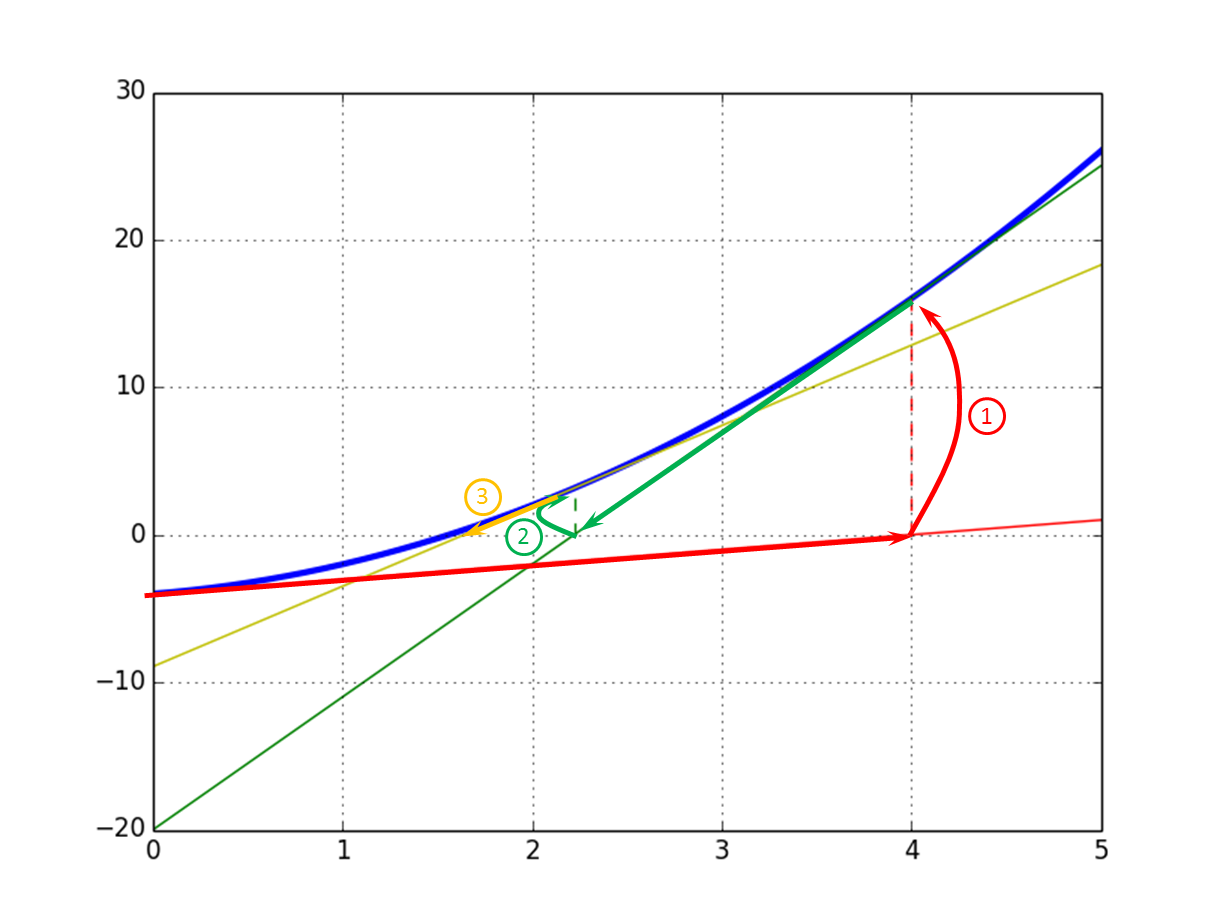
\includegraphics[width=\linewidth]{interpretation_newton}
\end{center}
\end{minipage}

\subsection*{Évaluation de la dérivée numérique}

\begin{resultat}
En première approximation, il est possible d'approximer la dérivée en approximant la tangente à la courbe par une droite passant par deux points successifs. Dans ces conditions, pour une valeur de $h$ suffisamment faible, on a : 
$$
f'(x_0)\simeq \dfrac{f(x_0+h)-f(x_0)}{h}.
$$
\end{resultat}


%
%\begin{resultat}
%\textbf{Théorème de Taylor-Young}
%Si $f$ est deux fois dérivable en $x_0$ et $f''(x_0)\neq 0$, 
%$$
% \dfrac{f(x_0+\varepsilon)-f(x_0)}{\varepsilon} - f'(x_0) \sim \dfrac{f''(x_0)}{2}h
%$$
%\end{resultat}%

\subsubsection{Méthodes à un pas}

\begin{minipage}[c]{.6\linewidth}
\begin{resultat}
\textbf{Différence avant -- Schéma d'Euler explicite}

Dans ce cas, l'estimation de la dérivée au point $P_i$ s'appuie sur le point $P_{i+1}$ :
$$
f'(x_i)\simeq\dfrac{f(x_{i+1})-f(x_i)}{x_{i+1}-x_i}
$$
\end{resultat}

\begin{resultat}
\textbf{Différence arrière -- Schéma d'Euler implicite}

Dans ce cas, l'estimation de la dérivée au point $P_i$ s'appuie sur le point $P_{i-1}$ :
$$
f'(x_i)\simeq\dfrac{f(x_{i})-f(x_{i-1})}{x_{i}-x_{i-1}}
$$
\end{resultat}
\end{minipage}\hfill
\begin{minipage}[c]{.35\linewidth}
\begin{center}
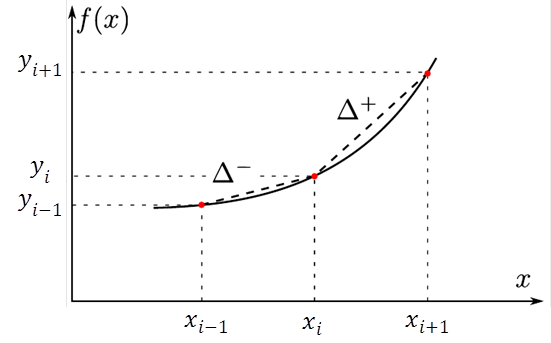
\includegraphics[width=\textwidth]{derivation_1pas}
\end{center}
\end{minipage}

\subsubsection{Méthode à deux pas}

\begin{minipage}[c]{.6\linewidth}
\begin{resultat}

On peut aussi utiliser les points $P_{i-1}$ et $P_{i+1}$ pour estimer la dérivée en $P_i$ :
$$
f'(x_i)\simeq\dfrac{f(x_{i+1})-f(x_{i-1})}{x_{i+1}-x_{i-1}}
$$

\end{resultat}

\begin{rem}
\begin{itemize}
\item Lorsqu'il s'agit de dériver une fonction temporelle « en temps réel », le point suivant n’est pas encore connu donc seule la différence arrière peut être calculée.
\item Le calcul de la dérivée conduit à un tableau de valeurs de dimension $n-1$.
\end{itemize}
\end{rem}
\end{minipage}\hfill
\begin{minipage}[c]{.35\linewidth}
\begin{center}
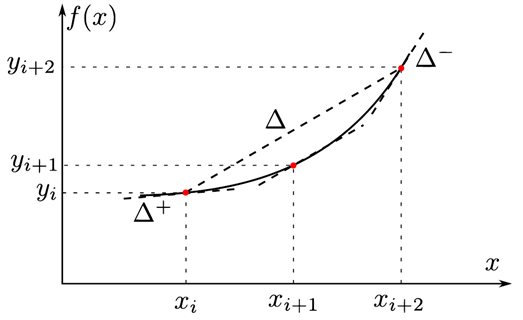
\includegraphics[width=\textwidth]{derivation_2pas}
\end{center}
\end{minipage}



\subsection{Bibliothèque Python}
Il est possible de résoudre l'équation $f(x)=0$ en utilisant les modules de la bibliothèque \texttt{scipy} :
\begin{py}
\begin{minipage}[c]{.45\linewidth}
Résolution de $\sin(x)=0$ avec 0,5 comme valeur d'initialisation.
\begin{lstlisting}
def f(x):
    return sin(x)
   
sol = newton(f,0.5)
print(sol)
print(f(sol))
\end{lstlisting}

Résolution du système : 
$$
\left\{\begin{array}{l} 
x+10y-3z-5 = 0 \\ 
2x-y+2z-2 = 0\\
 -x+y+z+3 = 0\end{array}\right.
 $$

\end{minipage}
\hfill
\begin{minipage}[c]{.45\linewidth}
\begin{lstlisting}
from scipy.optimize import fsolve
# définition du système
def syst(var): 
    # définition des variables
    x, y, z = var[0], var[1], var[2] 
    eq1 = x +10*y-3*z-5
    eq2 = 2*x-y+2*z-2
    eq3 = -x+y+z+3
    res = [eq1, eq2, eq3]
    return res
    # Initialisation de la recherche 
    # des solutions numériques
x0, y0, z0 = 0, 0, 0 
sol_ini = [x0, y0, z0]
sol = fsolve(syst, sol_ini)
sol = newton(f,0.5)
print(sol)
\end{lstlisting}
\end{minipage}

\end{py}


\section{Intégration numérique}

\begin{hypo}  $f:[a,b]\rightarrow \mathbb{R}$ est une fonction continue sur $[a,b]$. On note $I = \int\limits_a^{b} f(x) \mathrm{d}x $.
\end{hypo}

\subsection{Principe des méthodes des rectangles}
%\subsection{Principe}
\begin{defi}{Méthode des rectangles}
Dans cette méthode, la fonction à intégrer est interpolée par un polynôme de degré 0, à savoir une fonction constante. Géométriquement, l'aire sous la courbe est alors approximée par un rectangle. Plusieurs choix sont possibles.

\begin{minipage}[c]{.3\linewidth}
Rectangles à gauche :

$$
I = \int\limits_a^{b} f(x) \mathrm{d}x \simeq \left(b-a\right) f(a) 
$$
\end{minipage}\hfill
\begin{minipage}[c]{.3\linewidth}
Point milieu :

$$
I = \int\limits_a^{b} f(x) \mathrm{d}x \simeq \left(b-a\right) f\left(\dfrac{a+b}{2}\right) 
$$
\end{minipage}\hfill
\begin{minipage}[c]{.3\linewidth}
Rectangles à droite :

$$
I = \int\limits_a^{b} f(x) \mathrm{d}x \simeq \left(b-a\right) f(b) 
$$
\end{minipage}
\end{defi}

\subsection{Interprétation graphique}

\begin{minipage}[c]{.24\linewidth}
\begin{center}
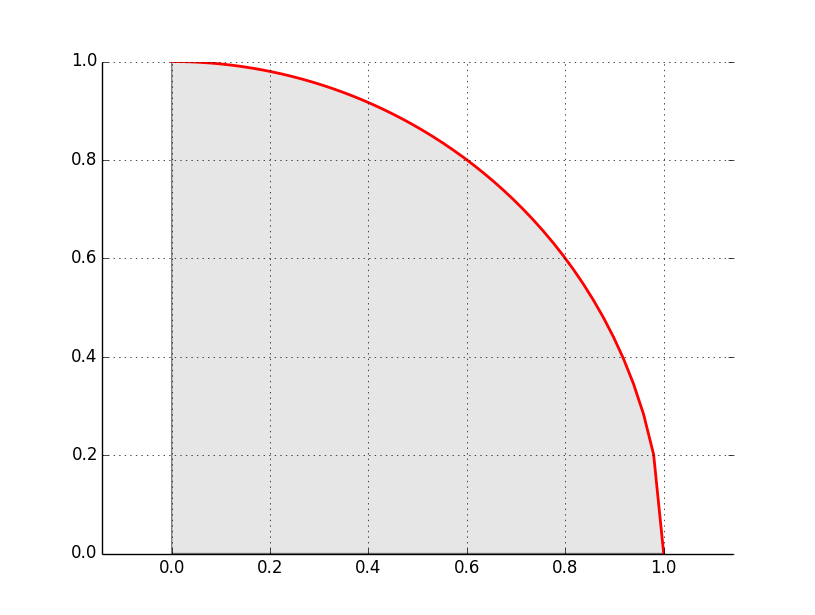
\includegraphics[width=.99\textwidth]{pi_courbe}

\textit{Calcul intégral}
\end{center}
\end{minipage}\hfill
\begin{minipage}[c]{.24\linewidth}
\begin{center}
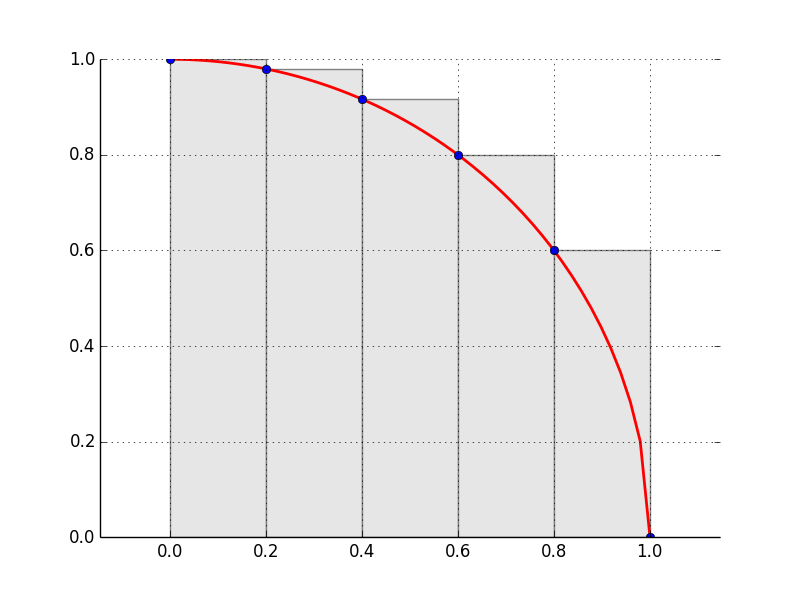
\includegraphics[width=.99\textwidth]{pi_rect_g}

\textit{Rectangles à gauche}
\end{center}
\end{minipage}\hfill
\begin{minipage}[c]{.24\linewidth}
\begin{center}
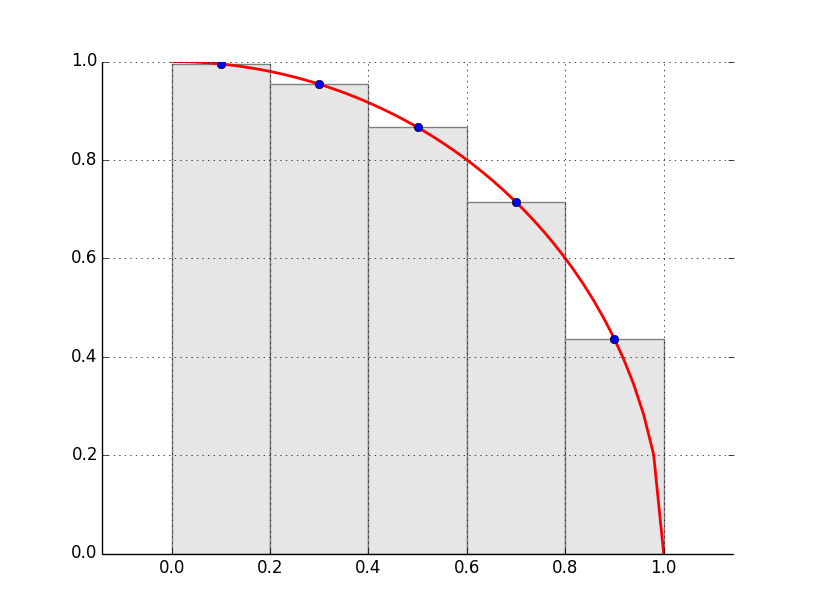
\includegraphics[width=.99\textwidth]{pi_rect_m}

\textit{Point milieu}
\end{center}
\end{minipage}\hfill
\begin{minipage}[c]{.24\linewidth}
\begin{center}
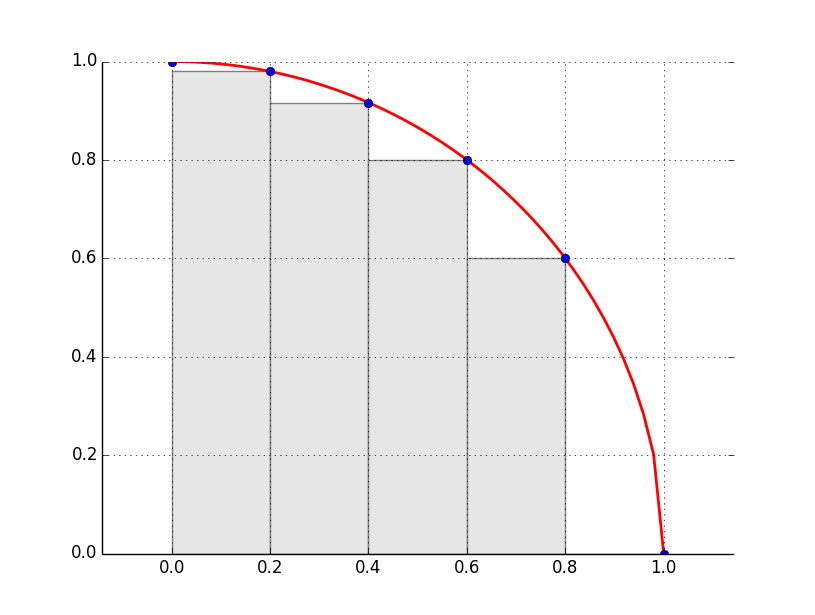
\includegraphics[width=.99\textwidth]{pi_rect_d}

\textit{Rectangles à droite}
\end{center}
\end{minipage}


\subsection{Principe des méthodes des trapèzes}
\begin{minipage}[c]{.7\linewidth}
\begin{defi}{Méthode des trapèzes}
Dans cette méthode, la fonction à intégrer est interpolée par un polynôme de degré 1, à savoir une fonction affine. Géométriquement, l'aire sous la courbe est alors approximée par un trapèze :

$$
I = \int\limits_a^{b} f(x) \mathrm{d}x \simeq \left(b-a\right) \dfrac{f(a)+f(b)}{2} 
$$
\end{defi}
\end{minipage}\hfill
\begin{minipage}[c]{.24\linewidth}
\begin{center}
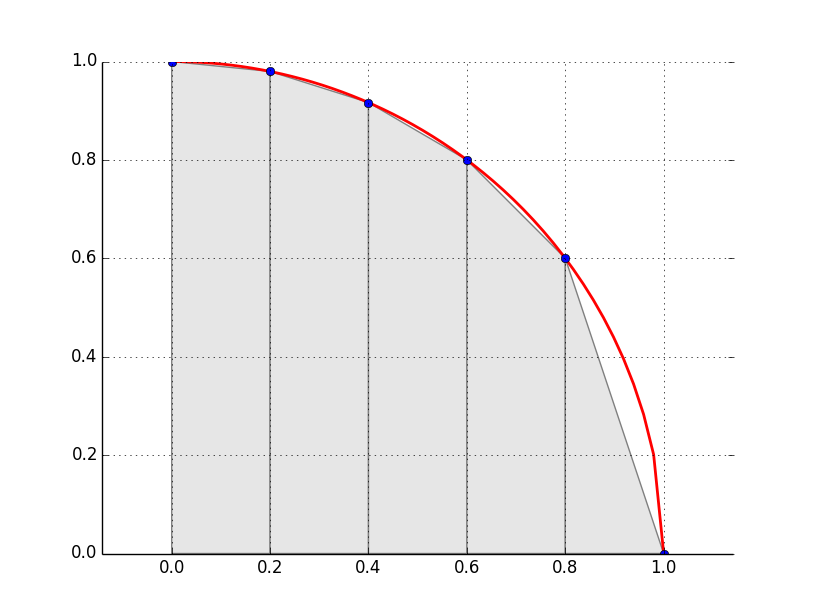
\includegraphics[width=.99\textwidth]{pi_trap}
\end{center}
\end{minipage}

\subsection*{Notion d'erreur d'intégration}
\begin{resultat}
Dans chaque cas,  on intègre $f$ sur $n$ subdivisions régulières de $I$. 

\textbf{Erreur sur la méthode des rectangles à gauche et à droite}

Soit $f$ fonction dérivable sur $I=[a,b]$ et dont $f'$ est continue sur $I$. Soit $M_1$ un majorant de $f'$ sur $I$. L'erreur $\varepsilon$ commise lors de l'intégration par la méthode des rectangles à droite ou à gauche
 est telle que $ \varepsilon \leq \dfrac{M_1}{2n}$.

\textbf{Erreur sur la méthode des rectangles -- point milieu}

Si de plus $f$ est deux fois dérivables sur $I=[a,b]$ et $f''$ est continue sur $I$, on note $M_2$ un majorant de $f''$ sur $I$.L'erreur $\varepsilon$ commise lors de l'intégration par la méthode des rectangles -- point milieu est telle que $ \varepsilon \leq \dfrac{M_2}{12n^2}$.

\textbf{Erreur sur la méthode des trapèzes}

L'erreur commise $\varepsilon$ est telle qu'il existe un entier $M$ tel que $ \varepsilon \leq \dfrac{M}{12n^2}$.

\end{resultat}

\subsection*{Bibliothèque Python}
Il est possible d'intégrer une fonction en utilisant les modules de la bibliothèque \texttt{scipy} :
\begin{lstlisting}
from scipy.integrate import quad
from math import sin
# Définition des bornes de gauche et de droite
g,d = -1,1 
def f(x):
    return sin(x)
   
I,erreur = quad(f,g,d)
print(I,erreur)
\end{lstlisting}


\section{Résolution d'équations différentielles}

\section{Résolution de systèmes linéaires}
